\documentclass{article}
\usepackage[T1]{fontenc}
\usepackage[a4paper, landscape]{geometry}
\usepackage{fontspec, graphicx, nopageno, tikz}

\usetikzlibrary{calc}
\pagenumbering{gobble}

\begin{document}

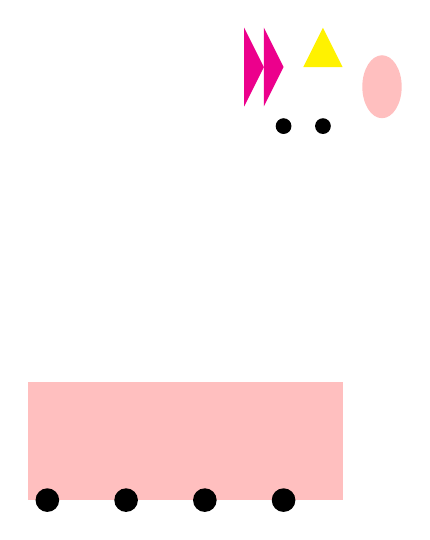
\begin{tikzpicture}[scale=0.5]

% Body
\fill[white] (0,0) circle (3);

% Head
\fill[white] (4,3) circle (2);

% Horn
\fill[yellow] (5,5) -- (4.5,6) -- (4,5) -- cycle;

% Eyes
\fill[black] (3.5,3.5) circle (0.2);
\fill[black] (4.5,3.5) circle (0.2);

% Ear
\fill[pink] (6,4.5) ellipse (0.5 and 0.8);

% Mane
\fill[magenta] (2.5,4) -- (3,5) -- (2.5,6) -- cycle;
\fill[magenta] (3,4) -- (3.5,5) -- (3,6) -- cycle;

% Legs
\fill[pink] (-1,-3) rectangle (1,-6);
\fill[pink] (1,-3) rectangle (3,-6);
\fill[pink] (3,-3) rectangle (5,-6);
\fill[pink] (-3,-3) rectangle (-1,-6);

% Hooves
\fill[black] (-0.5,-6) circle (0.3);
\fill[black] (1.5,-6) circle (0.3);
\fill[black] (3.5,-6) circle (0.3);
\fill[black] (-2.5,-6) circle (0.3);

\end{tikzpicture}
\vfill
\textcopyright 2024
\end{document}
